\section{Plateformes de développement}\label{hardware}
\renewcommand{\rightmark}{Plateformes de développement}
    Cette section décrit le matériel utilisé pour mettre en oeuvre la topologie décrite en
    \autoref{sec:archi-topologie}. Pour les racines RPL, la plateforme de développement Zolertia 
    RE-Mote Rev.B est utilisée, et, pour la racine LoRa, un Raspberry pi 3B+ est utilisé. 
    Leur interface LoRa est un RN2483. Les noeuds des réseaux RPL sont également la plateforme de 
    développement Zolertia RE-Mote Rev.B.

\subsection*{RN2483}\label{hardware:rn2483}
    Le RN2483 (Fig.~\ref{fig:state-rn2483}) est un modem LoRa compatible LoRaWAN$^{TM}$ basse énergie. D'après Nestor Ayuso~\cite{ayuso_2015}, il intègre un transceiver Semtech SX1276~\cite{sx1276:datasheet} et un microcontrôleur Microchip PIC18LF46K22.
    La communication avec ce modem est effetuée par des commandes ASCII envoyées via une interface UART. Il prend en charge les modulations FSK, GFSK et LoRa. Il possède également 14 GPIOs (General Purpose Input/Output).
    Ses fréquences opérationnelles sont situées dans les bandes 433 MHz et 868 MHz.
    D'après la datasheet~\cite{rn2483:datasheet}, 
    sa portée maximale est de 15km en agglomération et 5km en zone urbaine. Comme l'illustre la figure.~\ref{fig:state-rn2483}, pour ce mémoire, le RN2483 a été monté sur un carte d'interface réalisée par B.Quoitin qui comporte deux LEDs, une petite hélicoïdale ainsi que les connecteurs permettant d'utiliser des câbles de prototypages.

    \begin{figure}[H]
        \centering
        \includegraphics[scale=0.07]{res/pictures/monted_rn2483.png}
        \caption{RN2483.}
        \label{fig:state-rn2483}
    \end{figure}

    La figure \ref{fig:state-rn2484-block} reprend le schéma-bloc du RN2483. Il contient notamment l'interface UART, les antennes 433 MHz et 868Mhz ainsi que les GPIOs et la stack LoRaWan.
    \begin{figure}[H]
        \centering
        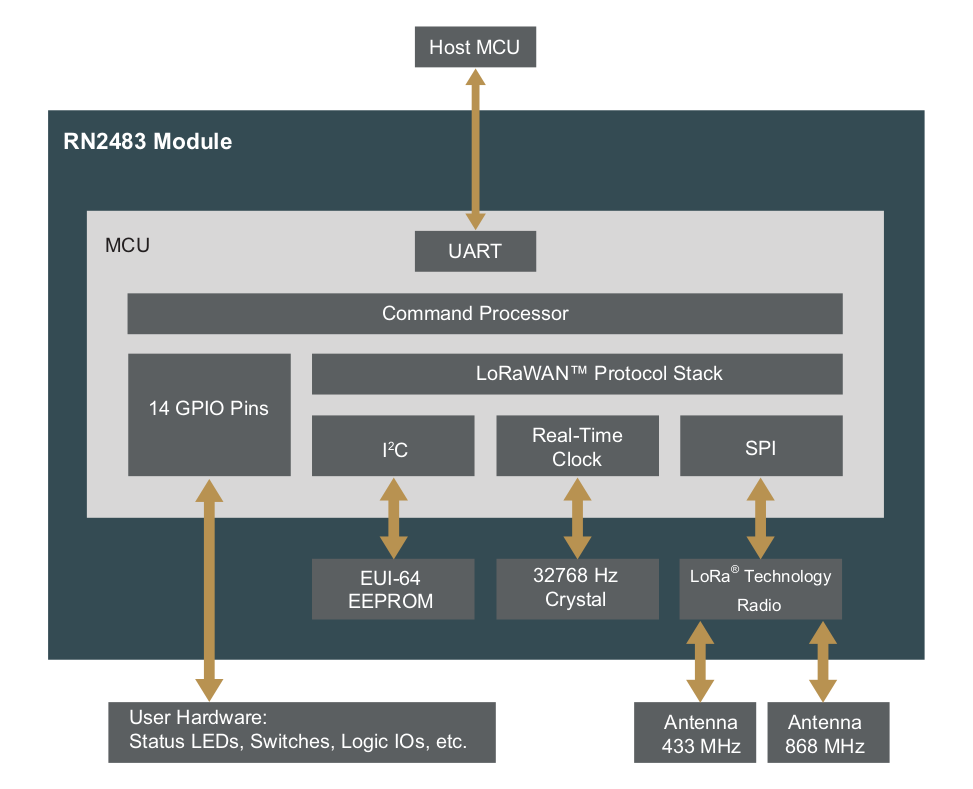
\includegraphics[scale=0.3]{res/pictures/rn2483-block-diagram.png}
        \caption{Schéma-bloc du RN2483~\cite{rn2483:datasheet}.}
        \label{fig:state-rn2484-block}
    \end{figure}

    La table~\ref{tb:state-rn2483-consumption} reprend la consommation électrique du RN2483 en fonction de son mode de fonctionnement pour alimentation de 3.3V qui est celle fournie par le RE-Mote et le Raspberry Pi.
    %\begin{table}[H]
    %    \centering
    %    \begin{tabular}{| *{4}{c|} }
    %        \hline
    %        Mode & \multicolumn{3}{c|}{\multirow{1}{*}{Courant (mA)}}\\ \cline{2-4}
    %         & VDD = 2.1V & VDD = 3.3V  & VDD = 3.6V \\ \hhline{|=|=|=|=|}
    %        Idle & 1.7 & 2.8 & 3.1 \\ \hline
    %        Transmit & 28.6 & 38.9 & 44.5 \\ \hline
    %        Sleep & 0.0015 & 0.0016 & 0.0016 \\ \hline
    %        Receive & 12.96 & 14.22 & 14.69 \\ \hline
    %    \end{tabular}
    %    \caption{Consommation de courant (à 25 °C) \cite{rn2483:datasheet}.}
    %    \label{tb:state-rn2483-consumption}
    %\end{table}
    \begin{table}[H]
        \centering
        \begin{tabular}{ | c | >{\centering\arraybackslash}p{2.5cm} | }
            \hline
            Mode & Courant(mA) \par VDD=3.3V \\ \hhline{|=|=|}
            Idle & 2.8 \\ \hline
            Transmit & 38.9 \\ \hline
            Sleep & 0.0016 \\ \hline
            Receive & 14.22 \\ \hline
        \end{tabular}
        \caption{Consommation de courant (à 25 °C) \cite{rn2483:datasheet}.}
        \label{tb:state-rn2483-consumption}
    \end{table}

\subsection*{Raspberry Pi}

Le Raspberri Pi est un ordinateur monocarte. Il possède notamment 40 pins GPIO, une interface Wi-Fi, Bluetooth, 4 ports USB 2.0 et un connecteur pour une caméra. Toutes ces caractéristiques en font une passerelle idéale pour ce projet. En effet, ils permettent d'utiliser plusieurs interfaces réseaux et d'y connecter des capteurs et actuateurs.

Le modèle utilisé pour ce projet est un Raspberry Pi 3 modèle B+ (Fig.~\ref{fig:state-raspberrypi}). Ce modèle est équipé d'un processeur quadri-coeur Broadcom BCM2837B0, Cortex-A53 64-bit SoC cadencé à 1.4GHz et embarque 1GB de mémoire RAM. 

La table \ref{tb:state-raspberrypi-spec} reprend les principales caractéristiques de ce modèle.

\begin{figure}[H]
    \centering
    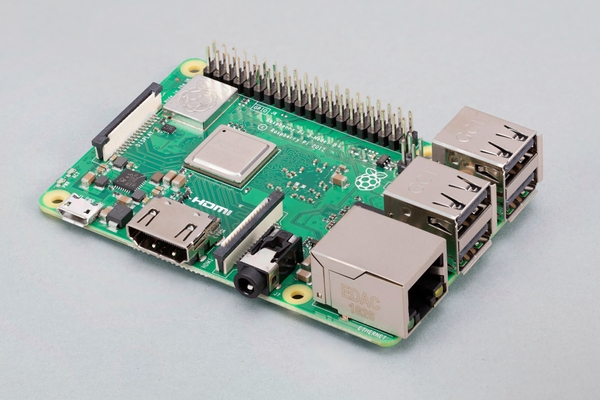
\includegraphics[scale=0.35]{res/pictures/raspberrypi3b+.png}
    \caption{Raspberry Pi 3B+~\cite{raspberry:shop}.}
    \label{fig:state-raspberrypi}
\end{figure}

\begin{table}[H]
    \centering
    \begin{tabular}{|c|p{0.75\textwidth}|}
        \hline
        \rowcolor{lightgray}
        Element            & Spécification\\
        CPU & Broadcom BCM2837B0, Cortex-A53 64-bit SoC à 1.4GHz\\ \hline
        Mémoire & 1GB LPDDR2 SDRAM \\ \hline
        Connectivité & 
        \begin{itemize}
            \item IEEE 802.11.b/g/n/ac, Bluetooth 4.2, BLE
            \item Gigabit Ethernet over USB 2.0
            \item 4 × USB 2.0 ports
        \end{itemize}\\ \hline
        Alimentation & 5V/2.5A DC\\ \hline
    \end{tabular}
    \caption{Spécifications du Raspberry Pi 3B+ \cite{raspberry:shop}.}
    \label{tb:state-raspberrypi-spec}
\end{table}

\subsection*{Zolertia RE-Mote}
Pour ce mémoire, la plateforme Zolertia RE-Mote Rev.B (Fig.~\ref{fig:state-zolertia}) est utilisée.
Cette plateforme, basée sur un system on chip (SoC) CC2538 ARM Cortex-M3, a été conçue par des universités et des industriels dans le but de permettre aux chercheurs et makers de développer des applications IoT et des objets connectés.

Le Zolertia RE-Mote a été choisi car il est équipé de deux radios compatibles IEEE 802.15.4,
permet une consommation électrique faible et possède de nombreux pins de connexion qui peuvent être utilisés pour y connecter des capteurs, actuateurs, radios, etc.

Le prix du constructeur pour cette plateforme est de 93,95€~\cite{zolertia-remote:shop}.

\begin{figure}[H]
    \centering
    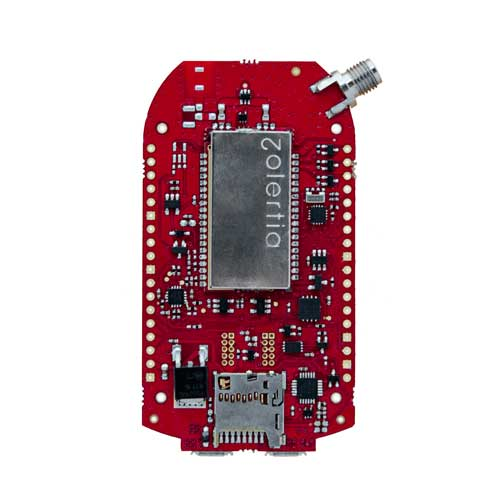
\includegraphics[scale=0.3]{res/pictures/remote-zolertia.jpg}
    \caption{Zolertia RE-Mote révision B~\cite{zolertia-remote:shop}.}
    \label{fig:state-zolertia}
\end{figure}

La table~\ref{tb:state-spec} reprend les principales spécifications du Zolertia RE-Mote rev.b.

\begin{table}[H]
    \centering
    \begin{tabular}{|c|p{8cm}|}
        \hline
        \rowcolor{lightgray}
        Element            & Spécification\\
        \hline
        Radio              & - IEEE 802.15.4 2.4 GHz \par - IEEE 802.15.4 863-950 MHz\\
        \hline
        CPU                & ARM\textsuperscript{\tiny\textregistered} Cortex\textsuperscript{\tiny\textregistered} -M3 jusqu'à 32 MHz\\
        \hline
        RAM                & 32 KB (16 KB pour tous les Power Modes)\\
        \hline
        Flash programmable & 512KB\\
        \hline
        I/O                & - RGB led, boutton user et reset \par - Slot Micro-SD \par - USB 2.0 à 12Mbps \par - Real-Time Clock\\
        \hline
    \end{tabular}
    \caption{Spécifications du Zolertia RE-Mote rev.b~\cite{zolertia-remote:datasheet}.}
    \label{tb:state-spec}
\end{table}

%todo connexion rn2483 -> rasp et re-mote